%% All structure, margins, title page, and packages live in upsgthesis.cls.
%% Language is selected here via the class option (english/czech); pass
%% 'twoside,openright' too for double-sided printing.
\documentclass[english,12pt,a4paper,twoside,openright]{upsgthesis}

%%% Thesis details
% Thesis title, in English (exactly as in the assignment)
\ThesisTitle{Thesis title}
% Thesis title, in Czech (exactly as in the assignment)
\ThesisTitleCZ{Název práce}

% Thesis type
\ThesisType{bachelor}
%\ThesisType{master}
%\ThesisType{rigorous}
%\ThesisType{dissertation}
%\ThesisType{lifelong}

% Author's name
\ThesisAuthor{Degree. First Last}

% Year of submission
\YearSubmitted{2026}

% Supervisor: first and last name with titles
\Supervisor{Degree. First Last}

% Study programme and branch
\StudyProgramme{Geology}

% Optional acknowledgements (to the supervisor, a consultant, whoever
% lent software, literature, etc.)
\Acknowledgements{%
I would like to thank the supervisor of my bachelor's thesis, [Degree. First Last, Degree], for their professional guidance, valuable advice, patience, and the time they devoted to me during the preparation of this thesis.
}

% Abstract (recommended length approx. 150-250 words; this is not the thesis assignment)
\Abstract{%
This bachelor's thesis deals with [main topic, e.g. the optimization of logistics processes in a selected company]. The aim of the thesis is to [clear aim, e.g. analyze the current state of warehouse management and propose measures to reduce costs]. The theoretical part summarizes key concepts and current knowledge in the field of [research field, e.g. lean logistics and inventory management]. In the practical part, [method, e.g. a financial and process analysis of the company XYZ is conducted using the ABC method]. Based on the identified shortcomings, which are mainly [main problems, e.g. a high error rate and inefficient goods placement], specific proposals for improvement are formulated in the conclusion of the thesis. The proposed solutions bring [contribution, e.g. a 15\% reduction in dispatch time and financial savings].
}
\AbstractCZ{%
Tato bakalářská práce se zabývá [hlavní téma práce, např. optimalizací logistických procesů ve vybrané firmě]. Cílem práce je [přesný cíl, např. analyzovat současný stav skladového hospodářství a navrhnout opatření ke snížení nákladů]. Teoretická část shrnuje klíčové pojmy a dosavadní poznatky v oblasti [oblast výzkumu, např. štíhlé logistiky a řízení zásob]. V praktické části je provedena [metoda, např. finanční a procesní analýza společnosti XYZ za využití metody ABC]. Na základě zjištěných nedostatků, kterými jsou zejména [hlavní problém, např. vysoká míra chybovosti a neefektivní rozmístění zboží], jsou v závěru práce formulovány konkrétní návrhy na zlepšení. Navržená řešení přinášejí [přínos, např. zkrácení doby expedice o 15\% a finanční úsporu].
}

% 3 to 5 keywords (recommended)
\Keywords{keyword, important term, another topic, and another one}
\KeywordsCZ{klíčové slovo, další pojem, jiný důležitý termín, a ještě jeden}

% Defaults to bibliography.bib; override with a different .bib file if needed.
%\Bibliography{bibliography.bib}

\begin{document}
%% Title page and various mandatory information pages
\thesisfrontmatter

\pagestyle{fancy}
%%% The individual thesis chapters are kept in separate files for clarity
\chapter*{Introduction}
\addcontentsline{toc}{chapter}{Introduction}

The introduction is a mandatory part of a bachelor's/master's thesis. The introduction is an introduction to the topic. It elaborates on the chosen topic, briefly places it in context (this may include a description of the motivation for writing the thesis), and answers the question of why the topic was chosen. It places the topic in context and justifies its necessity and the timeliness of addressing it. It contains an explicitly stated aim of the thesis. The text of the aim must match the text given in the thesis assignment, i.e. the text given in the SIS system, which is also given in the Abstract section.

The introduction also includes a brief presentation of how the thesis was processed (the processing method is covered in detail in a separate part of the main text). The introduction may also include a description of the motivation for writing the thesis.

The introduction to a master's thesis must be more elaborate -- see your faculty's thesis guidelines for details.

Several sample chapters follow, recommending how a final thesis should be typeset. They primarily describe the use of the \TeX{} template, but the general advice will also serve users of other systems well.

%%% Sample chapter with typesetting examples

\chapter{Typesetting Guide}

\section{Formatting the thesis}

The thesis text itself is organized hierarchically into chapters and sections, with each chapter starting on a new page. Text is justified. A new paragraph is usually separated by a small vertical space and indentation of the first line. The visual formatting should be consistent throughout the text.

Abbreviations used in the text must be explained at their first occurrence (in parentheses or in a footnote, if a more complex explanation of the term or abbreviation is needed). If there are many abbreviations, a list of abbreviations used should be added, including their explanation and/or references to their definition.

Longer text taken over from another author must be delimited with quotation marks or otherwise marked, and properly cited.

\section{Simple examples}

A narrow (non-breaking) space belongs between a number and a unit: the width of an A4 page is $210\,\rm mm$, which only $5\,\%$ of authors remember. But when the value is used attributively, the space is omitted: a $25\rm mm$ margin, a $95\%$ confidence interval.

We distinguish between different kinds of dashes:
red-black (hyphen),
pages 16--22 (en dash),
$45-44$ (mathematical minus),
and this is --- as you probably expected --- a parenthetical clause set off by em dashes.

Don't hard-code quotation marks with \texttt{``like this''}; use \verb|\enquote{like this}| instead. \enquote{Like this}, it automatically follows the typographic convention of whichever language babel is currently set to, so the same source works unchanged if the thesis language ever changes.

% This paragraph makes the tilde visible
{
\def~{{\tt\char126}}
In several places you need to prevent a line break (in \TeX{} we mark this with a tilde): between a number/letter and the unit or word that must stay with it -- vertex~$v$, in $k$~steps, Fig.~3, pp.~12--15, Ch.~5 -- and generally anywhere a line break would leave the reader \enquote{stumbling}, such as before a short word stranded at the start or end of a line.
}

%%% Sample chapter with examples of tables, figures, and code

\chapter{Tables, Figures, Code Listings}

Using tables and graphs/figures in academic text has some rules in common and some that are specific. We do not place tables and graphs/figures directly in the text, but on a separate page or in a reserved spot at the top or bottom of a normal page. \LaTeX\ takes care of the placement of floating graphs and tables automatically.

Graphs/figures and tables are numbered and carry a caption. The caption should describe the content of the graph or table in enough detail that the reader understands it without carefully studying the thesis text.

Every table and graph/figure must be referenced by number in the text (the dynamic cross-referencing mechanism built into \LaTeX\ is strongly recommended). At the relevant point in the text, summarize the most important conclusions that can be drawn from the table or graph. The text should be readable and understandable even without looking at the tables and graphs, and the tables and graphs should be understandable even without a detailed reading of the text.

Where possible, refer to tables and graphs indirectly as part of the normal flow of the text; instead of \emph{\enquote{Table~\ref{tab03:Estimates} shows that
    men are on average $9.9\,\rm kg$ heavier than women}} write
\emph{\enquote{Men are $9.9\,\rm kg$ heavier than women on average (see
    tab.~\ref{tab03:Estimates})}}.

\section{Tables}

\begin{table}[htbp!]

\centering
%%% This table uses the following packages:
%%%   - booktabs (\toprule, \midrule, \bottomrule)
%%%   - dcolumn (column type D: numbers centred and aligned on the
%%%     decimal point)

\caption{Maximum-likelihood estimates in model M.}\label{tab03:Estimates}
\begin{tabular}{lD{.}{.}{3.2}D{.}{.}{1.2}D{.}{.}{2.3}}
\toprule
               &                & \multicolumn{1}{c}{\textbf{Std.}}   &  \\
\textbf{Effect} & \multicolumn{1}{c}{\textbf{Estimate}} & \multicolumn{1}{c}{\textbf{error}$^a$} & \multicolumn{1}{c}{\textbf{P-value}} \\
\midrule
Intercept     & -10.01 & 1.01 & \multicolumn{1}{c}{---} \\
Sex (male)    & 9.89   & 5.98 & 0.098 \\
Height (cm)   & 0.78   & 0.12 & <0.001 \\
\bottomrule
\multicolumn{4}{l}{\footnotesize \textit{Note:}$^a$ Standard error of the estimate obtained by the Monte Carlo method.}
\end{tabular}
\end{table}

The following rules are recommended for \textbf{tables}:

\begin{itemize} %% or compactitem from the paralist package
\item Avoid vertical rules. Use heavier horizontal rules to separate
  the table from the surrounding text, including the caption, and
  lighter horizontal rules to separate the column headers from the
  body of the table and the individual parts of the table from each
  other. In \LaTeX\ this style of table is implemented by the
  \texttt{booktabs} package. If some columns need to be more clearly
  separated from others, insert a larger gap between them.
\item Do not change the type, format, or meaning of the content of
  cells within the same column (it is not good to put an average in
  one row of a column and a percentage in another).
\item Do not repeat the same cell content many times in a row. If we
  have a column \textit{Variance} that contains the value $0.5$ in
  the first ten rows and the value $1.5$ in the next ten rows, it is
  better to remove that column and solve it another way. For example,
  we can split the table into two, or insert descriptive rows that
  state some variable value that recurs across the following section
  of the table (e.g. \emph{\enquote{Variance${}=0.5$}} and below
  \emph{\enquote{Variance${}=1.5$}}).
\item Align numbers in a table on the decimal point.
\item A table sometimes needs to use abbreviations that do not occur
  elsewhere. These abbreviations can be explained in the caption or
  in notes below the table. Notes below the table can also be used to
  explain the meaning of certain columns or values in more detail.
\end{itemize}


\section{Figures}

\begin{figure}[htbp!]\centering
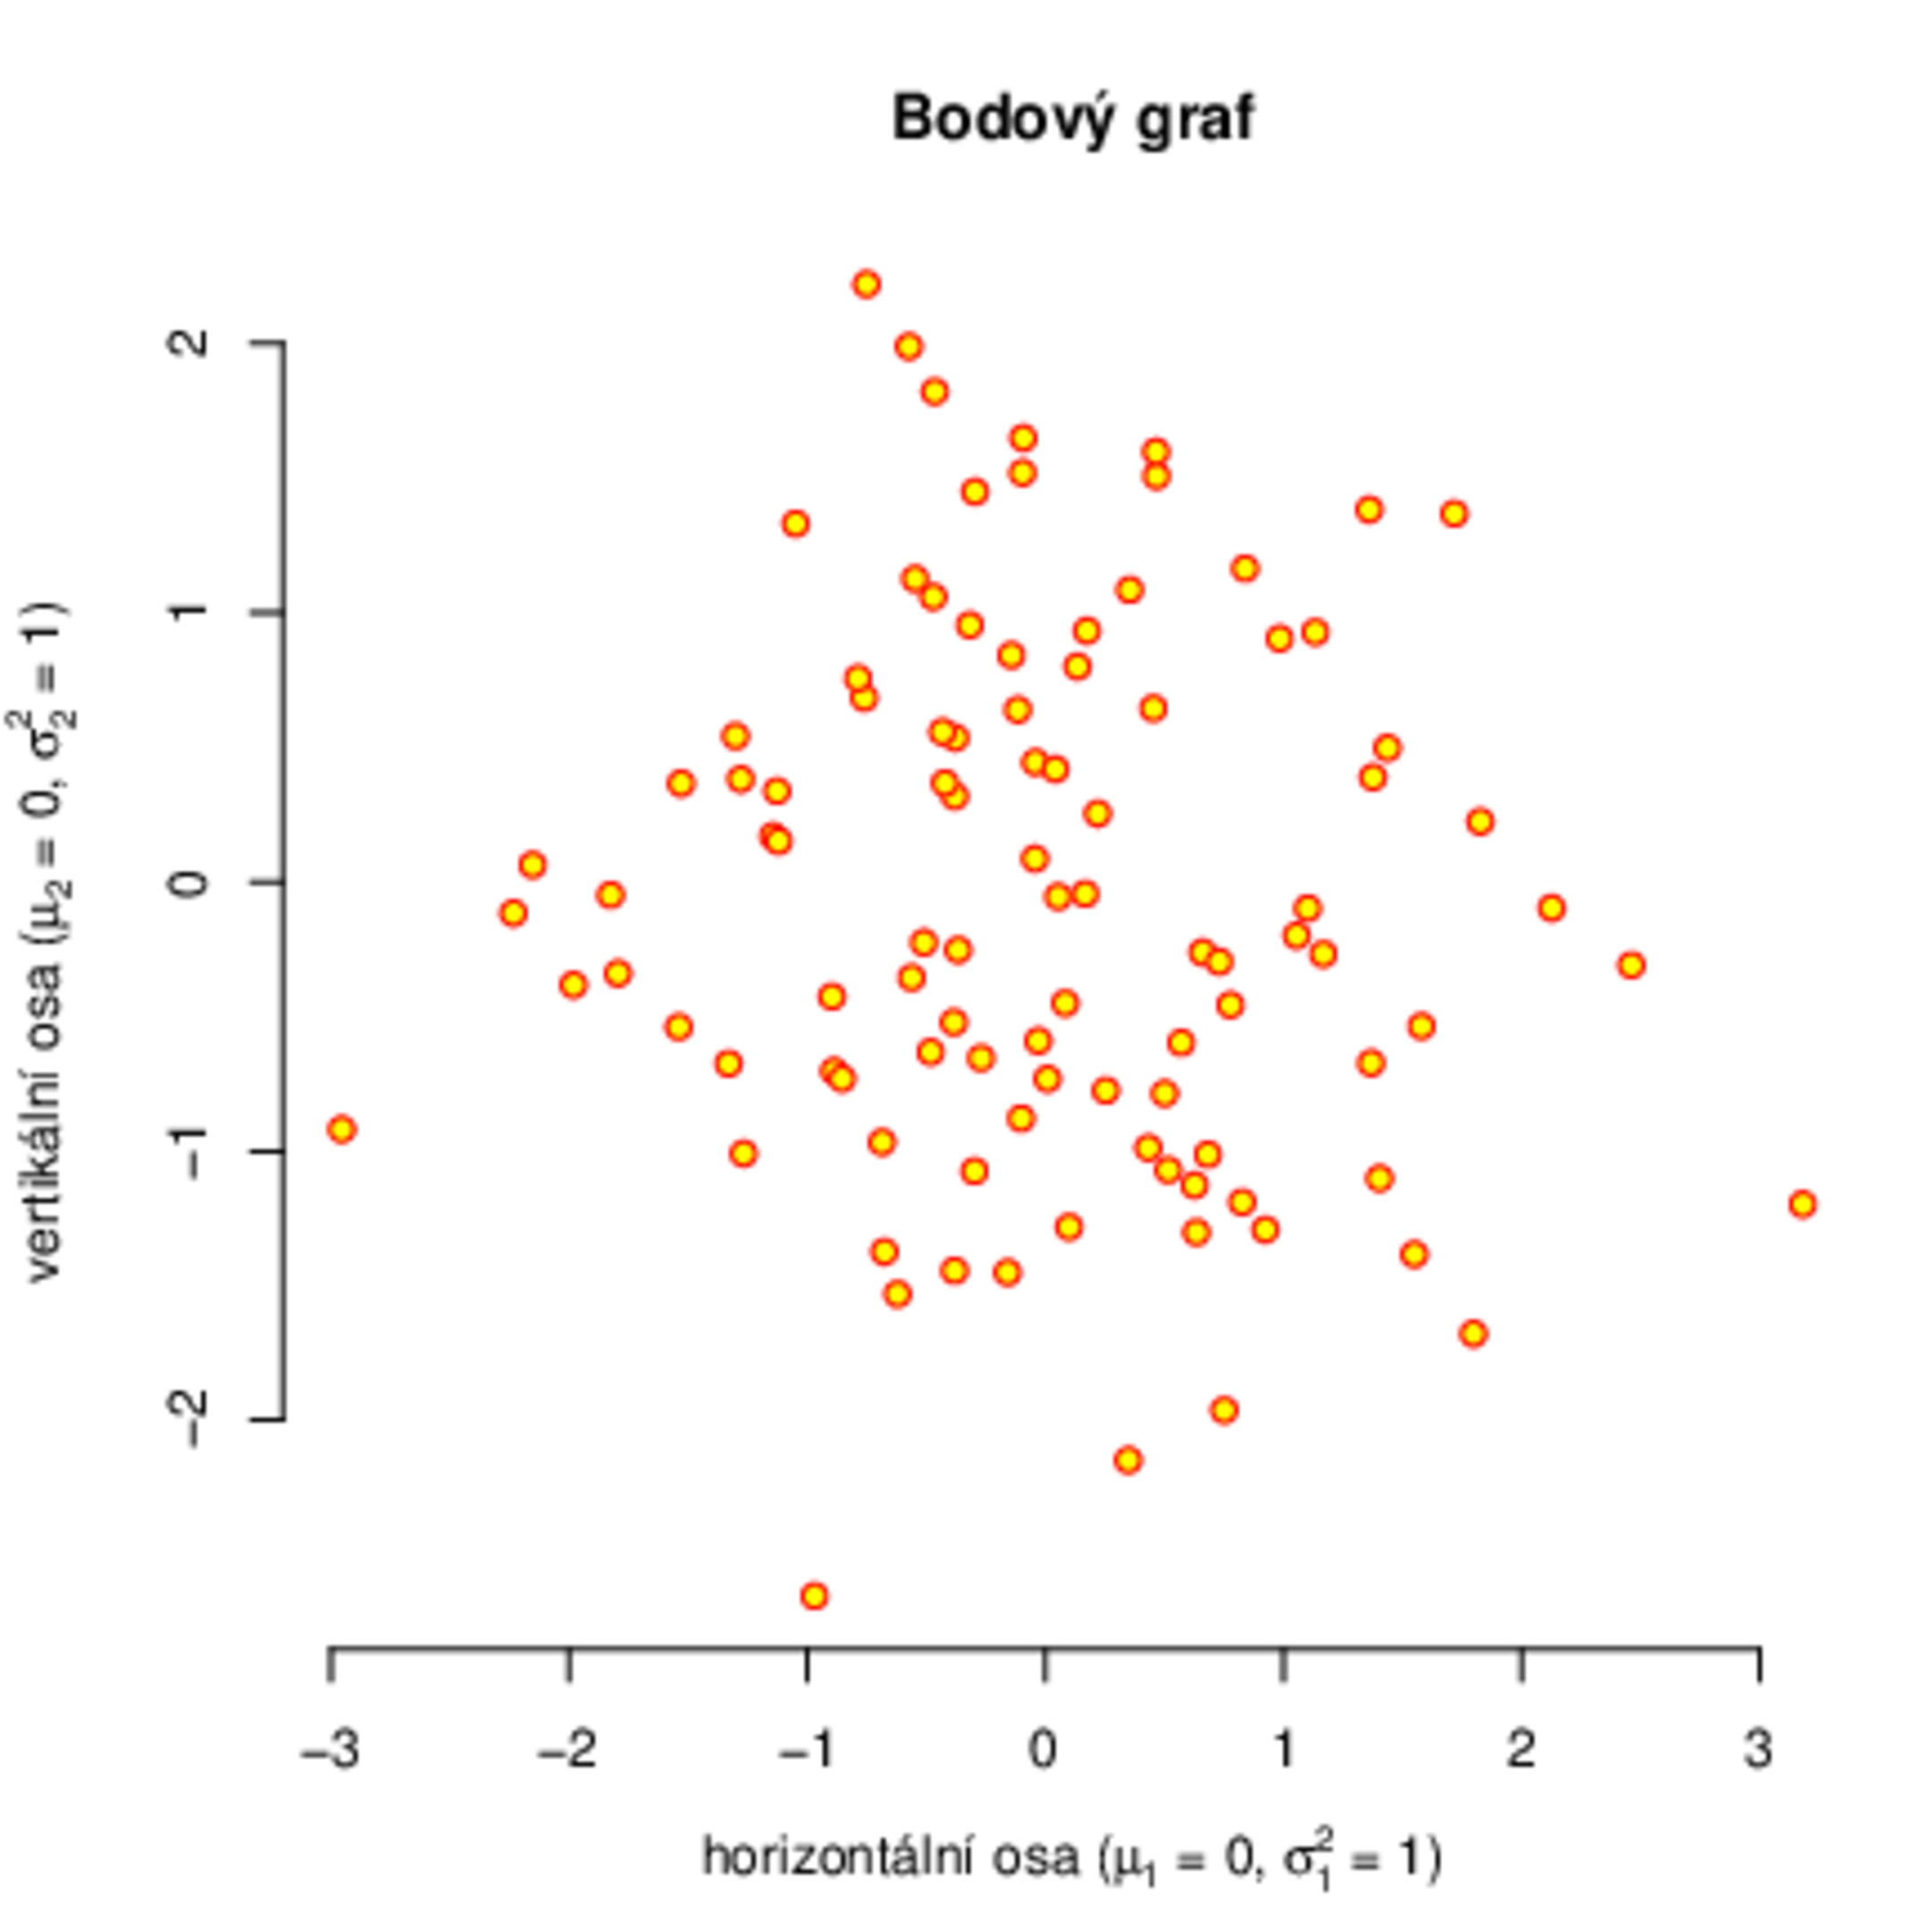
\includegraphics[width=.66\textwidth]{figures/example-fig01}
% There is no need to state the extension explicitly, pdflatex looks for a pdf automatically.
% There is also no need to state the dimensions.
\caption{A random sample from the distribution $\mathcal{N}_2(\boldsymbol{0},\,I)$.}
\label{fig03:Sample}
\end{figure}

A few pieces of advice regarding figures and graphs.

\begin{itemize}
\item A graph should be created at the size at which it will be used
  in the thesis. Shrinking a graph that is too large leads to poor
  label legibility.
\item The axes of a graph must be properly labelled in the same
  language the thesis is written in (missing diacritics can be
  tolerated). If plotting weight against height, don't leave the
  labels as \texttt{ht} and \texttt{wt}; instead label the axes
  \emph{Height [cm]} and \emph{Weight [kg]}. If plotting a function
  $h(x)$, label the axes $x$ and $h(x)$. Every axis must have a
  clearly defined scale.
\item If you need to mark a large number of points on a
  two-dimensional graph, make sure they do not merge into a solid
  black mass. If there are many points, reduce the size of the symbol
  used to plot them, or select only a small subset of the points to
  include in the graph. Graphs containing thousands of points cause
  problems especially in electronic documents, because they
  significantly increase file size.
\item If the thesis will be printed in black and white, avoid using
  colour. Distinguish lines by their style (solid, dotted,
  dash-dotted, \ldots), and areas by sufficiently different
  intensities of grey or by hatching. Explain the meaning of the
  individual line and area styles either in a text caption for the
  graph or in a graphical legend that is part of the figure itself.
\item Avoid low-resolution bitmap images, and JPEGs in particular
  (jagged edges and compression artefacts don't look good on paper).
  It is better to create images as vector graphics and insert them
  into the text as PDF (watch out for the PDF/A issue described in
  chapter~\ref{chap:pdfa}).
\end{itemize}


\section{Source Code}
Algorithms, program listings, and descriptions of program interaction are best set apart from the rest of the text. \texttt{upsgthesis.cls} defines a \texttt{code} environment on top of the \texttt{listings} package for this, with syntax highlighting for whichever language you name as its optional argument, e.g.\ \verb|\begin{code}[Python]|. Leave the argument out for plain, unhighlighted text -- useful for console transcripts such as the following. Longer or supplementary source code belongs in an appendix instead (see appendix~\ref{app:code}, which also shows a highlighted Python example).

\begin{code}
> mean(x)
[1] 158.90
> object$mean
[1] 158.90
\end{code}

\texttt{listings} is very richly configurable well beyond what this template sets up by default -- see its documentation, or:
\begin{itemize}
\item \url{https://en.wikibooks.org/wiki/LaTeX/Source_Code_Listings}
\item \url{https://www.overleaf.com/learn/latex/Code_listing#Using_listings_to_highlight_code}
\end{itemize}


\section{Typesetting Mathematics}
Variables are set in italics (\TeX{} does this automatically in math mode, but don't forget it in the surrounding text either, and remember to switch on math mode). Function names are set upright. For example:
$\textrm{var} (X) = \textsf{E~} X^2 - \bigl(\textsf{E~} X \bigr)^2$.

Fractions within a paragraph (such as $\frac{5}{7}$ or $\frac{x+y}{2}$) can be too cramped, so it is better to typeset simple fractions with a slash: $5/7$, $(x+y)/2$.

\LaTeX's options for typesetting mathematics are rich, but it is possible that in some specific situations they won't be sufficient. In that case, the American Mathematical Society (AMS) packages are recommended. The packages \texttt{amsmath}, \texttt{amsfonts}, and \texttt{amsthm} are loaded by default in \texttt{upsgthesis.cls}. To explore their capabilities further, see:
\begin{itemize}
\item Math Extension with AMS\LaTeX\ -- \url{http://ptgmedia.pearsoncmg.com/images/0321173856/samplechapter/kopkach15.pdf}
\item \url{https://www.overleaf.com/learn/latex/Aligning_equations_with_amsmath}
\item Math Mode -- \url{http://tex.loria.fr/general/Voss-Mathmode.pdf}
\item More Math into LaTeX -- \url{http://tug.ctan.org/info/Math_into_LaTeX-4/Short_Course.pdf}
\end{itemize}

%%% Sample chapter with citation examples

\chapter{Working with References}

The template assumes the use of a bibliography database for greater flexibility. Using a bibliography database is not a strict requirement; the standard \texttt{thebibliography} environment can also be used instead. In that case, however, the \texttt{upsgthesis.cls} class and main file need to be modified, as described below.

\section{Using a bibliography database}

\begin{enumerate}
\item\textbf{Changing the database name}\\
The template assumes a database stored in the file \texttt{bibliography.bib}. If the database has a different name, the value of the \verb'\addbibresource' command's parameter must be changed in \texttt{upsgthesis.cls}.
\item\textbf{Changing the citation style}\\
By default, citations in the text are given in numeric form. Switching to the surname-and-year combination is easy: change \texttt{upsgthesis.cls}, where you swap the comment character in the parameters for the \texttt{biblatex} package.
\end{enumerate}


\section{Using the \texttt{thebibliography} environment}
\begin{enumerate}
\item In \texttt{upsgthesis.cls}, delete these lines near the beginning:
\begin{verbatim}
%%% Settings for using a standalone bibliography database
\RequirePackage[
   backend=biber
  ,style=iso-authoryear %iso-numeric
  ,sortlocale=en_US
  ,bibencoding=UTF8
  %,block=ragged
]{biblatex}
\addbibresource{bibliography.bib}
\end{verbatim}
\item In \texttt{upsgthesis.cls}, edit the \verb'\thesisbibliography' command: remove the \verb'\printbibliography' call and replace it with the \texttt{thebibliography} environment.
\end{enumerate}


\section{How to Cite in the Text}
\begin{center}
\begin{tabular}{l@{~~$\longrightarrow$~~}l}
\verb|\cite{Cermak2018}|&\cite{Cermak2018}\\
\verb|\cite{Hladik2018,Jasek2018}|&\cite{Hladik2018,Jasek2018}\\
\verb|\cite[ch. 3]{Pecakova2018}|&\cite[ch. 3]{Pecakova2018}\\
\end{tabular}
\end{center}

%%% Sample chapter with PDF/A instructions

\chapter{The PDF/A Format}\label{chap:pdfa}

The electronic form of final theses
must be submitted in PDF/A format, level 1a or 2u. These are
profiles of the PDF format that determine which PDF features are permitted
to be used, so that documents are suitable for long-term archiving and
further automated processing. We will focus on level 2u, which we typeset with \TeX.

The most important requirements of PDF/A-2u include:

\begin{itemize}

\item All fonts must be embedded inside the document. References to
external fonts are not permitted (not even to \enquote{system} fonts such as Helvetica or Times).

\item Fonts must contain a ToUnicode table, which defines the mapping from the
character encoding used inside the font to Unicode. This makes it
possible to reliably extract text from the document.

\item The document must contain metadata in XMP format, and if it is in
colour, also a formal specification of the colour space.

\end{itemize}

This template uses the {\tt pdfx} package, which can configure \LaTeX{}
to satisfy the PDF/A requirements. The XMP metadata is generated automatically from the
information in the file matching your main file's name, e.g. {\tt thesis-en.xmpdata} (you can look at the
generated file in {\tt pdfa.xmpi}).

PDF/A validity can be checked using an online validator: \url{https://www.pdf-online.com/osa/validate.aspx/}.

If the file is not valid, common causes include the use of less common
fonts (which are embedded only in bitmap form and/or without Unicode
tables) and the inclusion of images in PDF that do not themselves conform to
the PDF/A standard.

This is likely to affect images created by many different programs.
In such a case, you can try to convert the image to PDF/A using
GhostScript, for example like this:

\begin{verbatim}
        gs -q -dNOPAUSE -dBATCH
           -sDEVICE=pdfwrite -dPDFSETTINGS=/prepress
           -sOutputFile=output.pdf input.pdf
\end{verbatim}

% \include{...}
% \include{...}
\chapter*{Conclusion}
\addcontentsline{toc}{chapter}{Conclusion}

The conclusion is a mandatory part of a bachelor's/master's thesis. It contains a summary of the thesis and addresses the extent to which the aim set out in the thesis was achieved, or summarizes the answers to the questions posed in the introduction of the thesis.

The conclusion of a master's thesis must be more elaborate -- see your faculty's thesis guidelines for details.

The conclusion is treated as a chapter that starts on a separate page and is titled Conclusion. The title Conclusion is not numbered. The text of the conclusion itself is organized into paragraphs.


%%% List of references used
\thesisbibliography

%%% Appendices to the thesis, if any. Every appendix must be referenced at
%%% least once from the main text. Appendices are numbered.
\thesisappendices
\chapter{Source Code}\label{app:code}

The following Python command-line script reads waypoints from a GPX file and adds them as sites to an SDB database, illustrating a typical short data-processing utility.

\begin{code}[Python]
from typing import Annotated
import typer
from gpx import read_gpx
from apsg.database import SDBSession


def format_name(name):
    prefix = "".join(c for c in name if not c.isdigit())
    suffix = "".join(c for c in name if c.isdigit())
    return f"{prefix}{int(suffix):03d}"


def main(
    sdb: Annotated[str, typer.Argument(help="path of SDB database.")],
    file: Annotated[str, typer.Argument(help="path of GPX file.")],
    fixname: bool = False,
):
    """
    Add sites from gpx file to SDB

    Examples:
        $ add_from_gpx.py dest.sdb file.gpx
        $ add_from_gpx.py dest.sdb file.gpx --fixname

    """
    db = SDBSession(sdb)
    gpx = read_gpx(file)
    unit = db.unit("Default")
    for wpt in gpx.wpt:
        site = db.site(
            wpt.name,
            unit=unit, x_coord=float(wpt.lon), y_coord=float(wpt.lat)
        )
        print(f"{site} added")

    confirm = input("OK? [y/N] ")
    if confirm in ["Y", "y"]:
        db.commit()
        db.close()
        print("Done.")
    else:
        print("Canceled.")


if __name__ == "__main__":
    typer.run(main)
\end{code}

% \include{...}
% \include{...}

\end{document}
